\section{Kurzschlussversuch}
Für den Kurzschlussversuch werden die sekundärseitigen Klemmen allpolig kurzgeschlossen (siehe Abbildung\;\ref{fig:Kurzschluss_Messschaltung}) und zusätzlich der sekundärseitige Kurzschlussstrom $I_{K,S}$ gemessen.
\begin{figure}
    \centering
    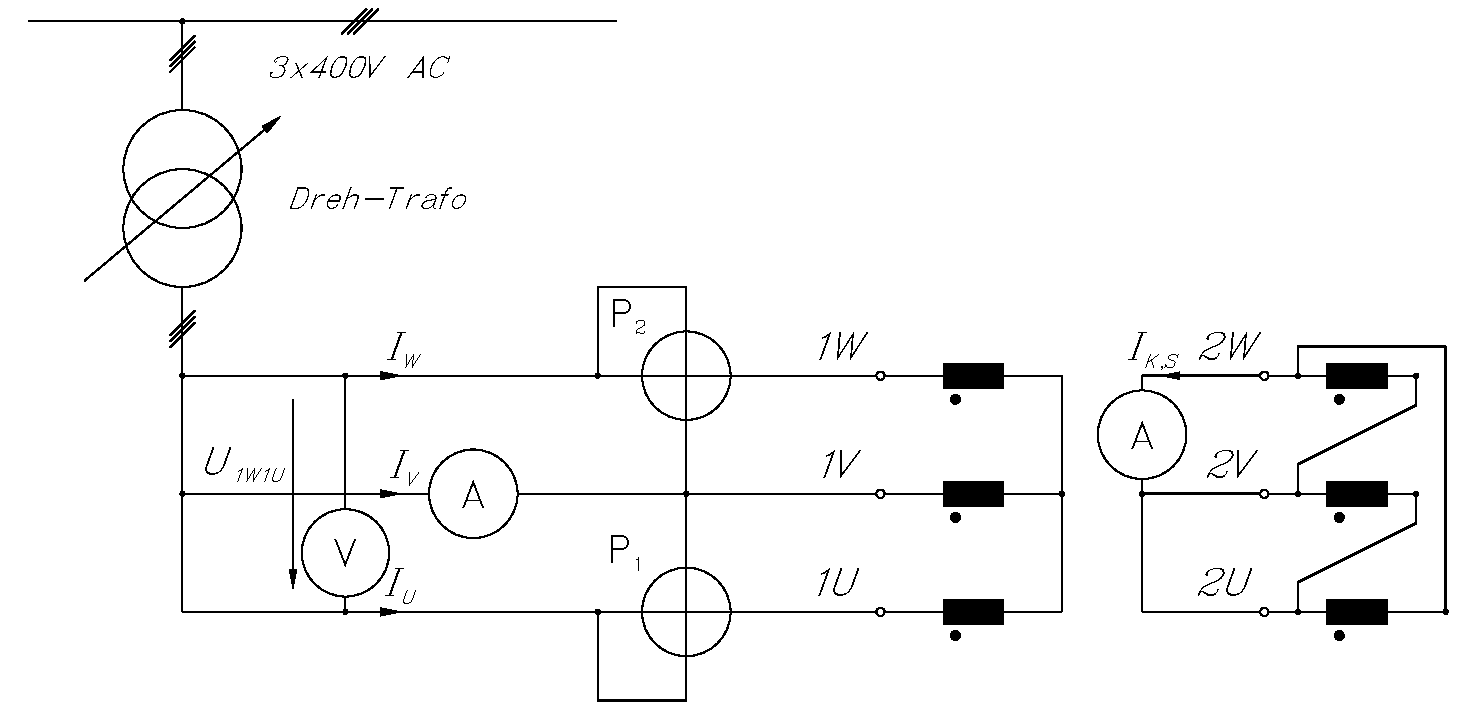
\includegraphics[width=0.75\textwidth]{\currfiledir images/Kurzschluss}
    \caption{Messschaltung für die Ermittlung der Kenngrößen im Kurzschlussfall (primärseite Aussenleiterspannungen und Aussenleiterströme bzw. aufgenommene Wirkleistung und sekundärseitiger Kurzschlussstrom)}
    \label{fig:Kurzschluss_Messschaltung}
\end{figure}\\
\noindent
Da die Kurzschlussspannung nur wenige Prozent ($\approx5\%$) der Nennspannung beträgt, wird bereits bei ca. $5\%$ der Primär-Nennspannung der Nennstrom fließen. Deshalb, und auch um den Einschaltstromstoß zu minimieren, wird der kurzgeschlossene Transformator bei annähernd $\SI{0}{\volt}$ Eingangsspannung in Betrieb genommen. Sodann wird diese sukzessive erhöht, bis der 1,2 fache Nennstrom fließt und danach aus thermischen Gründen (ähnliche Wicklungstemperatur für die gesamte Messung), die Messung mit fallender Eingangsspannung durchgeführt. Tabelle \ref{tab:kurzschluss} listet die Messwerte auf.\\

\begin{table}[ht!]
    \centering% Tabelle zu kurzschluss.csv
    \begin{tabular}{|c|c|c|c|c|}
    \hline
    \bfseries $I_k[\SI{}{\ampere}]$ & \bfseries $P_k[\SI{}{\watt}]$ & \bfseries $S_k[\SI{}{VA}]$ & \bfseries $U_k[\SI{}{\volt}]$ & \bfseries $\mathrm{cos}(\varphi_k)[\SI{}{1}]$
    \csvreader[head to column names]{4/kurzschluss.csv}{}
    {\\\hline\csvcoli& \csvcolii& \csvcoliii& \csvcoliv& \csvcolv}
    \\\hline
    \end{tabular}
    \caption{Messwerte zum Kurzschlussversuch}
    \label{tab:kurzschluss}
\end{table}

\noindent Aus den Messergebnissen können verschiedene Parameter des Transformators bestimmt werden. Neben der Kurzschlussimpedanz $Z_K$ und deren Komponenten, auch die Kurzschlussspannung und der Dauerkurzschlussstrom bzw. die Kupferverluste.\\
Aus der Messung der drei Primär-Strangströme bzw. der verketteten Primär-Spannungen (und anschließender Mittelwertbildung) wurde der Kurzschlussstrangstrom bzw. die Primär-Strangspannung errechnet, woraus der Betrag der Kurzschlussimpedanz bestimmt werden kann:
\begin{equation}
\begin{split}
    Z_k & = \frac{U_k/\sqrt{3}}{I_k} = \frac{\SI{11.3}{\volt}}{\SI{78.07}{\ampere}} = \SI{0.144}{\ohm}\\
    R_k & = \cos(\varphi)\cdot Z_k = 0.39\cdot \SI{0.144}{\ohm}=\SI{0.0563}{\ohm}\\
    X_k & = \sqrt{Z_k^2\,-\,R_k^2}=\SI{0.133}{\ohm}
\end{split}
\end{equation}
und mit der Bezugsgröße der Impedanz
\begin{equation}
    Z_{Bezug} = \frac{\hat{U}_{N,S}}{\hat{I}_{N,S}}=\frac{\SI{311}{\volt}}{\SI{107}{\ampere}}=\SI{2.895}{\ohm}
\end{equation}
kann diese auch in normierter Form angegeben werden (inkl. Komponenten)
\begin{equation}
\begin{split}
    z_k = u_k & = \frac{Z_k}{Z_{Bezug}}=\frac{\SI{0.144}{\ohm}}{\SI{2.895}{\ohm}}=0,04989\approx5\%\\
    r_k = u_r & = \frac{R_k}{Z_{Bezug}}=\frac{\SI{0.0563}{\ohm}}{\SI{2.895}{\ohm}}=0,0195\\
    x_k = u_x & = \frac{X_k}{Z_{Bezug}}=\frac{\SI{0.133}{\ohm}}{\SI{2.895}{\ohm}}=0,0459.
\end{split}
\end{equation}
Der Dauerkurzschlussstrom ist definiert, als jener Strom der theoretisch fließen würde, wenn an den sekundärseitig kurzgeschlossenen Transformator, primärseitig Nennspannung anliegen würde. Er berechnet sich daher aus der bezogenen Kurzschlussspannung zu:
\begin{equation}
    I_{k,D}=\frac{I_{N,S}}{u_k}=\frac{\SI{76}{\ampere}}{0,04989}=\SI{1523}{\ampere}.
\end{equation}
Die Bestimmung der Kupferverluste im Nennpunkt erfolgt durch den Zusammenhang zwischen dem Strangstrom und Nennpunkt $I_{N,S}$ und dem ohmschen Anteil der Kurzschlussimpedanz $R_k$ (bei Wicklungstemperatur = Raumtemperatur $\approx\,25^{\circ}C$):
\begin{equation}
    P_{N,Cu,25^{\circ}C}=3\cdot I_{N,S}^2\cdot R_{k,25^{\circ}C} = 3\cdot (\SI{76}{\ampere})^2\cdot \SI{0.0563}{\ohm}=\SI{976}{\watt}
\end{equation}
Durch die Temperaturabhängigkeit des Wicklungswiderstandes (Temperaturkoeffizient von Kupfer, $\alpha_{Cu}=0,00393$), folgt bei erhöhter Wicklungstemperatur auch eine Erhöhung des Wicklungswiderstandes
\begin{equation}
    R_{k,75^{\circ}C}=R_{k,25^{\circ}C}\,[1+\alpha_{Cu}\,(75^{\circ}C-25^{\circ}C)]=\SI{0.0563}{\ohm}\cdot 1,1965=\SI{0.0673}{\ohm}
\end{equation}
und damit der Kupferverluste im Nennpunkt (bei $75^{\circ}C$ Wicklungstemperatur)
\begin{equation}
    P_{N,Cu,75^{\circ}C}=3\cdot I_{N,S}^2\cdot R_{k,75^{\circ}C} = 3\cdot (\SI{76}{\ampere})^2\cdot \SI{0.0673}{\ohm}=\SI{1168}{\watt}.
\end{equation}
Abbildung\;\ref{fig:Kurzschluss_Strom} zeigt den Zusammenhang zwischen Strangstrom und Aussenleiterspannung. Aufgrund der geringen Eingangsspannung befindet sich der Transformator noch nicht in Sättigung und deshalb im unteren, linearen Bereich seiner Kennlinie (linearer Zusammenhang zwischen Strangstrom und Strang-/Aussenleiterspannung).\\
Ebenfalls ein linearer Zusammenhang besteht zwischen dem Quadrat der Eingangsspannung und der vom Transformator aufgenommenen Wirk- und Scheinleistung, bzw. ein quadratischer Zusammenhang, wenn die Strang-/Aussenleiterspannung linear skaliert wird (siehe Abbildung\;\ref{fig:Kurzschluss_Leistung}). Da die Spannung am Querzweig des Ersatzschaltbildes (Abb.\;\ref{fig:Leerlauf_ESB_1straengig}) ebenfalls sehr klein ist (ungefähr halbe Aussenleiterspannung), ist der Einfluss der Hauptreaktanz bzw. Eisenverlustwiderstandes vernachlässigbar, was sich auch in einem konstantem Verlauf des Leistungsfaktors $\cos(\varphi)$ äußert.
\input{\currfiledir kurzschluss_strom}
\input{\currfiledir kurzschluss}
\clearpage
